% SC2001 --- Chapter 1: Foundations (0->100 ground-up)
\chapter{Foundations: From Zero to Algorithmic Reasoning}
\label{ch:foundations}

\begin{quote}
\emph{``An algorithm must be seen to be believed.''} --- Donald Knuth. Before we design faster algorithms, we must agree on what an algorithm \emph{is}, how to argue that it is \emph{correct}, and what it costs to run. This chapter builds that floor from first principles.
\end{quote}

\noindent\fbox{\parbox{\dimexpr\linewidth-2\fboxsep-2\fboxrule}{%
\textbf{From zero: we build here, no MH1812/SC1007 needed.} This chapter defines every discrete-math notion from scratch---sets, functions, logic, sums, proofs, induction---with pictures before formalism. No prior discrete math or data-structures course is assumed. Later chapters depend only on what is built here.}}
\vspace{0.4em}

\section*{Learning Outcomes}
After this chapter you will be able to:
\begin{enumerate}[label=(L\arabic*)]
    \item recall essential discrete-mathematical notation and handle sums, logarithms, floors and ceilings fluently;
    \item distinguish and apply direct proof, contrapositive, contradiction, and counterexamples;
    \item prove statements by (weak and strong) mathematical induction;
    \item define \emph{algorithm} precisely and describe the RAM model and its cost measure;
    \item prove correctness of iterative algorithms using loop invariants and termination arguments.
\end{enumerate}

% ============================================================
\section{Discrete Mathematics Refresher}
\label{sec:discrete-refresher}
We collect notation used throughout the book---built from zero, not assumed from MH1812. Each idea appears as picture $\to$ words $\to$ definition.

% --- 2 TikZ BEFORE formal sets/functions (audit L30) ---
\begin{figure}[h]
\centering
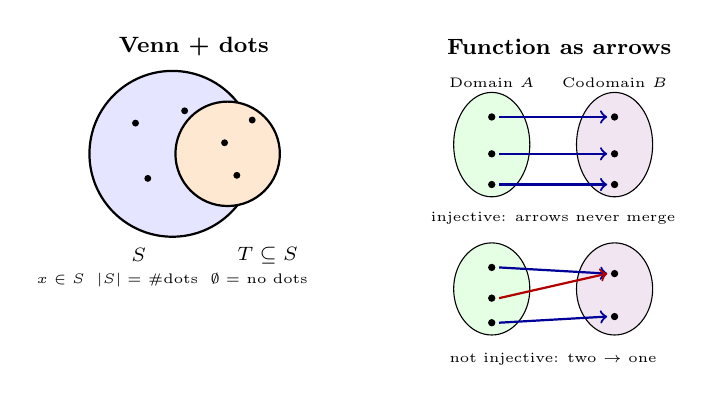
\begin{tikzpicture}[scale=0.78,every node/.style={font=\scriptsize}]
% Venn + dots for \in,\subseteq,|S|
\begin{scope}
\draw[thick,fill=blue!10] (0,0) circle (1.35);
\draw[thick,fill=orange!18] (0.9,0) circle (0.85);
\foreach \x/\y in {-0.6/0.5,-0.4/-0.4,0.2/0.7,0.85/0.18,1.05/-0.35,1.3/0.55} \fill (\x,\y) circle (1.6pt);
\node at (-0.55,-1.65) {$S$}; \node at (1.55,-1.65) {$T\subseteq S$};
\node[font=\tiny] at (0,-2.05) {$x\in S$\; $|S|=$ \#dots\; $\emptyset=$ no dots};
\node[font=\footnotesize\bfseries] at (0.35,1.75) {Venn + dots};
\end{scope}
% Arrow domain->codomain: injective vs non-injective
\begin{scope}[xshift=5.2cm]
\node[font=\footnotesize\bfseries] at (1.1,1.75) {Function as arrows};
% injective
\draw[rounded corners=3pt,fill=green!10] (0,0.15) ellipse (0.62 and 0.85);
\draw[rounded corners=3pt,fill=violet!10] (2.0,0.15) ellipse (0.62 and 0.85);
\node[font=\tiny] at (0,1.15) {Domain $A$}; \node[font=\tiny] at (2.0,1.15) {Codomain $B$};
\foreach \y/\yy in {0.6/0.6,0.0/0.0,-0.5/-0.5} {\fill (0,\y) circle (1.7pt); \fill (2.0,\yy) circle (1.7pt); \draw[->,thick,blue!60!black] (0.12,\y)--(1.88,\yy);}
\node[font=\tiny,fill=white,inner sep=1pt] at (1.0,-1.05) {injective: arrows never merge};
% non-injective below
\begin{scope}[yshift=-2.35cm]
\draw[rounded corners=3pt,fill=green!10] (0,0.15) ellipse (0.62 and 0.75);
\draw[rounded corners=3pt,fill=violet!10] (2.0,0.15) ellipse (0.62 and 0.75);
\foreach \y in {0.5,0.0,-0.4} \fill (0,\y) circle (1.7pt);
\foreach \y in {0.4,-0.3} \fill (2.0,\y) circle (1.7pt);
\draw[->,thick,blue!60!black] (0.12,0.5)--(1.88,0.4);
\draw[->,thick,red!70!black] (0.12,0.0)--(1.88,0.4);
\draw[->,thick,blue!60!black] (0.12,-0.4)--(1.88,-0.3);
\node[font=\tiny,fill=white,inner sep=1pt] at (1.0,-1.0) {not injective: two $\to$ one};
\end{scope}
\end{scope}
\end{tikzpicture}
\caption{Left: sets as dot collections inside Venn ovals. Right: a function is arrows domain$\to$codomain; injective means no two arrows share a target.}
\label{fig:sets-functions}
\end{figure}

\subsection{Sets, Functions, Relations}
A \emph{set} is an unordered collection of distinct objects. We write $x\in S$, $S\subseteq T$, $S\subsetneq T$, $|S|$ for cardinality, $\emptyset$ for the empty set, $\mathbb{N}=\{0,1,2,\dots\}$ (we include $0$), $\mathbb{Z},\mathbb{Q},\mathbb{R},\mathbb{Z}^+$.
A \emph{function} $f:A\to B$ assigns to each $a\in A$ exactly one $b=f(a)\in B$. $A$ is the domain, $B$ the codomain, $f(A)=\{f(a):a\in A\}$ the image. $f$ is \emph{injective} if $f(a)=f(a')\Rightarrow a=a'$, \emph{surjective} if $f(A)=B$, \emph{bijective} if both. Composition $(g\circ f)(a)=g(f(a))$.
A \emph{relation} $R\subseteq A\times A$ may be reflexive, symmetric, transitive, antisymmetric---yielding equivalences and partial orders. A \emph{graph} $G=(V,E)$ with $E\subseteq V\times V$ is used from Ch.~6; we define paths/cycles/trees when first needed (no SC1007 assumed).

\subsection{Logic and Quantifiers}
\emph{Everyday first.} ``Every student passed'' vs.\ ``Some student passed'' already contain the two quantifiers. Picture a row of dots (students); colour a dot green if it satisfies property $P$.
\begin{center}
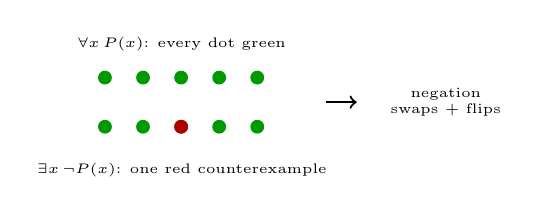
\begin{tikzpicture}[scale=0.78,every node/.style={font=\scriptsize}]
\foreach \i in {0,...,4} {\fill[green!60!black] (\i*0.62,0.45) circle (3.2pt); \fill[green!60!black] (\i*0.62,-0.35) circle (3.2pt);}
\fill[red!70!black] (2*0.62,-0.35) circle (3.2pt);
\node[font=\tiny] at (1.25,1.0) {$\forall x\,P(x)$: every dot green};
\node[font=\tiny] at (1.25,-1.05) {$\exists x\,\neg P(x)$: one red counterexample};
\draw[->,thick] (3.6,0.05)--(4.1,0.05);
\node[font=\tiny,align=center] at (5.55,0.05) {negation\\swaps + flips};
\end{tikzpicture}
\end{center}
Formally, propositions combine via $\neg,\land,\lor,\Rightarrow,\Leftrightarrow$. Quantifiers $\forall$ (\emph{for all}) and $\exists$ (\emph{there exists}) bind variables: $\forall n\in\mathbb{N},\,P(n)$ and $\exists x\in S,\,Q(x)$. Swapping gives De Morgan:
\[
\neg(\forall x\,P(x))\equiv\exists x\,\neg P(x),\qquad
\neg(\exists x\,P(x))\equiv\forall x\,\neg P(x).
\]
``Not every student passed'' $\equiv$ ``Some student failed''---swap $\forall\leftrightarrow\exists$ and flip $P\to\neg P$. Implication $P\Rightarrow Q\equiv\neg P\lor Q\equiv(\neg Q\Rightarrow\neg P)$ (contrapositive).

\subsection{Sums, Products, Logarithms}
We build each closed form from a picture, then state it. Each box is a 3-line derivation.
\paragraph{Arithmetic $1+2+\cdots+n=n(n+1)/2$ (Gauss pairing).}
Pair $1+n=n+1$, $2+(n-1)=n+1$, \dots---$n/2$ pairs. Two staircases make an $n\times(n+1)$ rectangle.
\begin{center}
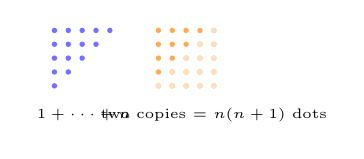
\begin{tikzpicture}[scale=0.55]
\foreach \i in {1,...,5} {\foreach \j in {1,...,\i} \fill[blue!55] (\j*0.32,\i*0.32) circle (1.8pt);}
\foreach \i in {1,...,5} {\foreach \j in {1,...,5} \fill[orange!65] (2.4+\j*0.32,\i*0.32) circle (1.8pt);}
\foreach \i in {1,...,5} {\foreach \j in {\i,...,5} \fill[orange!25] (2.4+\j*0.32,\i*0.32) circle (1.8pt);}
\node[font=\tiny] at (1.0,-0.35) {$1+\cdots+n$}; \node[font=\tiny] at (4.0,-0.35) {two copies = $n(n+1)$ dots};
\end{tikzpicture}
$\displaystyle\sum_{i=1}^{n}i=n(n+1)/2$.
\end{center}
\paragraph{Geometric $1+r+\cdots+r^{n-1}=(r^n-1)/(r-1)$ (binary tree).}
Level $i$ has $r^i$ nodes; stack levels form a tree. Multiply by $(r-1)$ telescopes. If $|r|<1$, $\sum_{i\ge0}r^i=1/(1-r)$.
\begin{center}
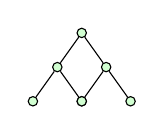
\begin{tikzpicture}[scale=0.62,level distance=7mm,sibling distance=10mm,every node/.style={circle,draw,fill=green!18,inner sep=1.2pt,font=\tiny}]
\node {} child {node {} child {node {}} child {node {}}} child {node {} child {node {}} child {node {}}};
\end{tikzpicture}
\ {\scriptsize $1+r+r^2+\cdots$ as tree levels; $r=2$ doubles each row.}
\end{center}
$\displaystyle\sum_{i=0}^{n-1}r^i=(r^n-1)/(r-1)$.
\paragraph{Harmonic $H_n=\sum_{i=1}^{n}1/i=\ln n+\gamma+O(1/n)$ (coupon/stack).}
$H_n$ is area of $n$ bars width $1$, height $1/i$---sandwiched between $\int_1^{n+1}\!dx/x$ and $1+\int_1^n\!dx/x$. Hence $\ln(n+1)\le H_n\le1+\ln n$; limit $\gamma\approx0.5772$.
\paragraph{Logarithms (rulers).} $\log$ without base $=\log_2$ for algorithms; $\ln=\log_e$, $\lg=\log_2$ always. Change of base is rescaling a ruler: $\log_a n=(\log_b n)/(\log_b a)=\Theta(\log_b n)$---base irrelevant inside $O(\cdot)$.
\paragraph{Floors/ceilings (number line, off-by-one $\le1$).}
\begin{center}
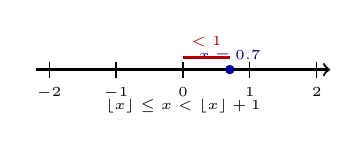
\begin{tikzpicture}[scale=0.85]
\draw[->,thick] (-2.2,0)--(2.2,0);
\foreach \x in {-2,-1,0,1,2} {\draw (\x,0.12)--(\x,-0.12) node[below,font=\tiny] {$\x$};}
\fill[blue!60!black] (0.7,0) circle (2pt) node[above,font=\tiny] {$x=0.7$};
\draw[thick,red!70!black] (0,0.18)--(0.7,0.18) node[midway,above,font=\tiny] {$<1$};
\node[font=\tiny] at (0,-0.55) {$\lfloor x\rfloor\le x<\lfloor x\rfloor+1$};
\end{tikzpicture}
\end{center}
$\lfloor x\rfloor\le x<\lfloor x\rfloor+1$, $\lceil x\rceil-1<x\le\lceil x\rceil$, $x-1<\lfloor x\rfloor\le x\le\lceil x\rceil<x+1$---dropping $\lfloor\cdot\rfloor$ errs by at most $1$.
Also $n!\le n^n$, $2^n\le n!$ for $n\ge4$, $(1+1/n)^n<e<(1+1/n)^{n+1}$.
\begin{example}[Manipulating sums]
For $n\ge1$, $\sum_{i=1}^{n}(2i-1)=2\frac{n(n+1)}2-n=n^2$ by linearity $\sum c a_i=c\sum a_i$, $\sum(a_i+b_i)=\sum a_i+\sum b_i$.
\end{example}

% ============================================================
\section{Proof Techniques}
\label{sec:proofs}
Every correctness proof uses one of four patterns.
\begin{definition}[Theorem, Lemma, Corollary]
A \emph{theorem} is a statement proved true. A \emph{lemma} is a helper theorem; a \emph{corollary} is an immediate consequence.
\end{definition}
\subsection{Direct Proof} Assume hypothesis; deduce conclusion.
\begin{example} If $n$ odd then $n^2$ odd. \emph{Proof.} $n=2k+1\Rightarrow n^2=4k^2+4k+1=2(2k^2+2k)+1$ odd. \qed \end{example}
\subsection{Contrapositive} Prove $\neg Q\Rightarrow\neg P$ instead of $P\Rightarrow Q$.
\begin{example} If $n^2$ even then $n$ even. Contrapositive: if $n$ odd then $n^2$ odd---proved above. \qed \end{example}
\subsection{Proof by Contradiction} Assume false, derive $R\land\neg R$.
\begin{example}[Irrationality of $\sqrt2$] If $\sqrt2=p/q$ lowest terms, $2q^2=p^2\Rightarrow p$ even $=2k\Rightarrow q^2=2k^2\Rightarrow q$ even---contradicts $\gcd(p,q)=1$. \qed \end{example}
\subsection{Counterexample and Cases} To disprove $\forall x\,P(x)$ give one $x$ with $\neg P(x)$; to prove by cases exhaust all possibilities.
\begin{example} ``Every $n>1$ prime'' false: $4=2\cdot2$. ``$n^2\bmod4\in\{0,1\}$'': even $n=2k\Rightarrow4k^2\equiv0$; odd $n=2k+1\Rightarrow4k(k+1)+1\equiv1$. \end{example}
\begin{remark}[How to choose] Try direct first. If conclusion is a negation (``not'', ``irrational'', ``no algorithm''), try contradiction. If $P$ itself is negated, contrapositive is often direct in disguise. \end{remark}

% ============================================================
\section{Mathematical Induction}
\label{sec:induction}
Induction proves loop invariants, recurrence closed forms, and properties of recursive structures.
\subsection{Weak Induction} To prove $\forall n\ge n_0,\,P(n)$: (I1) base $P(n_0)$; (I2) $\forall k\ge n_0,\,P(k)\Rightarrow P(k+1)$. $P(k)$ is the IH.
\begin{theorem}[Sum of first $n$ integers] For $n\ge1$, $\sum_{i=1}^{n}i=n(n+1)/2$. \end{theorem}
\begin{proof} Base $1=1\cdot2/2$. IH $\sum_{i=1}^{k}i=k(k+1)/2$. Then $\sum_{i=1}^{k+1}i=k(k+1)/2+(k+1)=(k+1)(k+2)/2$. \end{proof}
\subsection{Strong Induction} Assume all $P(j)$, $n_0\le j\le k$, to get $P(k+1)$.
\begin{theorem}[Every $n\ge2$ has a prime divisor] For $n\ge2$, $n$ divisible by a prime. \end{theorem}
\begin{proof} Base $2$ prime. Fix $k\ge2$, assume every $2\le j\le k$ has a prime divisor. If $k+1$ prime done; else $k+1=a\cdot b$, $2\le a,b\le k$, prime divisor of $a$ divides $k+1$. \end{proof}
\begin{theorem}[Fibonacci growth] $F_0=0,F_1=1,F_n=F_{n-1}+F_{n-2}\Rightarrow F_n\ge2^{n/2-1}$ for $n\ge1$. \end{theorem}
\begin{proof} Bases $n=1,2$ check. IH for $1\le j\le k$, $k\ge2$: $F_{k+1}=F_k+F_{k-1}\ge2^{k/2-1}+2^{(k-1)/2-1}\ge2^{(k+1)/2-1}$ since $\sqrt2+1>2$. \end{proof}
\subsection{Structural Induction} For recursively defined sets (lists, trees), prove base structures and that constructors preserve $P$.
\begin{example}[Binary trees] Tree is $\mathsf{Leaf}$ or $\mathsf{Node}(L,x,R)$. To prove ``leaves $=$ internal $+1$'' for full trees, check leaf base and show constructor preserves invariant. \end{example}

% ============================================================
\section{What Is an Algorithm?}
\label{sec:what-is-algorithm}
\begin{definition}[Algorithm, informal] A finite, unambiguous sequence of elementary steps that, given any admissible input, terminates and produces the required output. \end{definition}
Knuth's five criteria: finiteness, definiteness, input, output, effectiveness---plus termination on every admissible input. A procedure that may loop forever is a computational method, not an algorithm. An algorithm is distinct from a program: the idea vs.\ its realisation in Python/Java/C with the same asymptotics.
\subsection{Pseudocode Conventions} Language-agnostic, one-indexed arrays (CLRS style), \texttt{//} comments, $\gets$, $=,\neq,<,\le$, \texttt{if--then--else}, \texttt{while}, \texttt{for}, \texttt{return}. Count primitive ops (\S\ref{sec:ram}) not wall-clock time.
\begin{example}[Euclid --- oldest non-trivial algorithm]
\begin{quote}\ttfamily\scriptsize
\textsc{Euclid}$(a,b)$ // assume $a\ge b\ge0$\\
1\ \ \textbf{while} $b\neq0$ \textbf{do}\\
2\ \ \ \ \ \ $r \gets a \bmod b$\\
3\ \ \ \ \ \ $a \gets b$\\
4\ \ \ \ \ \ $b \gets r$\\
5\ \ \textbf{return} $a$
\end{quote}
We prove in \S\ref{sec:invariants} this returns $\gcd(a,b)$ and in Ch.~2 it costs $O(\log\min(a,b))$ divisions.
\end{example}

% ============================================================
\section{The Random Access Machine (RAM) Model}
\label{sec:ram}
To compare algorithms fairly we need a shared cost model: the Random Access Machine, an idealised von Neumann computer.
\begin{figure}[h]
\centering
\resizebox{\linewidth}{!}{%
\begin{tikzpicture}[
  box/.style={draw, thick, rounded corners=3pt, fill=blue!5, minimum height=0.9cm, align=center, font=\small},
  memcell/.style={draw, thick, minimum width=1.0cm, minimum height=0.55cm, font=\scriptsize, align=center},
  arrow/.style={-{Latex}, thick, color=violet!70!black},
  tape/.style={draw, thick, minimum width=0.55cm, minimum height=0.7cm, font=\scriptsize, align=center}
]
\fill[yellow!10,rounded corners=3pt] (-6.35,0.82) rectangle (-3.2,1.58);
\node[font=\footnotesize\bfseries] at (-5.2,2.0) {Input tape};
\foreach \i in {0,...,4} {\node[tape, fill=yellow!15] at (-6.0+\i*0.62,1.2) {};}
\node[font=\scriptsize] at (-6.0,1.2) {$x_1$}; \node[font=\scriptsize] at (-5.38,1.2) {$x_2$}; \node[font=\scriptsize] at (-4.76,1.2) {$\cdots$}; \node[font=\scriptsize] at (-4.14,1.2) {$x_n$}; \node[tape, fill=gray!20] at (-3.52,1.2) {\#};
\node[box, minimum width=3.6cm, minimum height=3.2cm, fill=blue!7, draw=blue!60!black] (cpu) at (0,0) {};
\node[font=\footnotesize\bfseries] at (0,1.25) {CPU};
\node[box, minimum width=3.0cm, minimum height=0.6cm, fill=orange!18] (ctrl) at (0,0.65) {Control Unit + Program Counter};
\node[box, minimum width=1.35cm, minimum height=0.7cm, fill=green!15] (regs) at (-0.73,-0.25) {Registers\\{\scriptsize $R_0\ldots R_k$}};
\node[box, minimum width=1.35cm, minimum height=0.7cm, fill=red!12] (alu) at (0.73,-0.25) {ALU\\{\scriptsize $+,-,\times,\div$}};
\node[box, minimum width=3.0cm, minimum height=0.45cm, fill=blue!10] (fetch) at (0,-1.05) {\scriptsize Fetch--Decode--Execute cycle};
\fill[blue!4,rounded corners=4pt] (3.65,-2.15) rectangle (5.55,1.75);
\node[font=\footnotesize\bfseries] at (4.6,2.0) {Memory (RAM)};
\foreach \i/\addr in {0/0,1/1,2/2,3/3,4/4} {\pgfmathsetmacro{\y}{1.15 - \i*0.60}\node[memcell, fill=blue!5] at (4.6,\y) {};\node[font=\tiny, anchor=east] at (3.85,\y) {\addr};}
\node[font=\scriptsize] at (4.6,1.15) {$M[0]$}; \node[font=\scriptsize] at (4.6,0.55) {$M[1]$}; \node[font=\scriptsize] at (4.6,-0.05) {$M[2]$}; \node[font=\scriptsize] at (4.6,-0.65) {$\vdots$}; \node[font=\scriptsize] at (4.6,-1.25) {$M[m-1]$}; \node[font=\tiny, align=center] at (4.6,-1.95) {random access\\in $O(1)$};
\fill[yellow!10,rounded corners=3pt] (-6.35,-3.42) rectangle (-3.75,-2.68);
\node[font=\footnotesize\bfseries] at (-5.2,-2.3) {Output tape};
\foreach \i in {0,...,3} {\node[tape, fill=yellow!15] at (-6.0+\i*0.62,-3.05) {};}
\node[font=\scriptsize] at (-6.0,-3.05) {$y_1$};
\draw[arrow] (-4.4,1.2) -- (-1.8,0.6) node[midway, above, font=\tiny] {read};
\draw[arrow] (1.8,0.35) -- (3.7,0.55) node[midway, above, font=\tiny] {load};
\draw[arrow] (3.7,-0.05) -- (1.8,-0.35) node[midway, below, font=\tiny] {store};
\draw[arrow] (-1.8,-0.6) -- (-4.4,-3.05) node[midway, below, font=\tiny] {write};
\draw[arrow, thin] (regs) -- (alu); \draw[arrow, thin] (alu) -- (regs);
\node[font=\tiny, align=center, fill=orange!15, rounded corners=2pt, inner sep=2pt] at (0,-2.05) {each primitive op costs $1$};
\end{tikzpicture}}%
\caption{The RAM. CPU fetches via program counter, operates on registers/ALU, accesses any $M[i]$ in unit time.}
\label{fig:ram-model}
\end{figure}
Concretely: memory $M[0\ldots m-1]$ of words ($\Theta(\log n)$ bits) with $O(1)$ random access; CPU registers + ALU + program counter; instruction set \texttt{LOAD}, \texttt{STORE}, \texttt{ADD}, \texttt{SUB}, \texttt{MUL}, \texttt{DIV}, \texttt{MOD}, \texttt{COMPARE}, \texttt{JUMP}, \texttt{JZ}, \texttt{READ}, \texttt{WRITE} each cost $1$ (uniform cost); program stored separately.
\subsection{Cost Model and Word-RAM Refinement}
Running time $=$ number of primitive steps. Input size in words (or bits when bit-complexity matters). Uniform cost suffices while numbers fit in a word ($w=\Theta(\log n)$ bits). For huge integers, arithmetic on $b$-bit values costs $\Theta(b/w)$; we flag when bit-complexity matters.
Why this model? It abstracts caches/pipelines yet predicts correctly: $O(n\log n)$ beats $O(n^2)$ past a modest $n$, letting us reason before implementing.
\begin{example}[Cost of linear search]
\begin{quote}\ttfamily
\textsc{LinearSearch}$(A,n,key)$\\
1\ \ \textbf{for} $i\gets1$ \textbf{to} $n$ \textbf{do}\\
2\ \ \ \ \ \ \textbf{if} $A[i]=key$ \textbf{then return} $i$\\
3\ \ \textbf{return} NIL
\end{quote}
Each iteration does $O(1)$ RAM ops (array access + compare + branch); time $\propto$ iterations $=O(n)$ worst-case.
\end{example}

% ============================================================
\section{Correctness: Loop Invariants and Termination}
\label{sec:invariants}
An algorithm is useless if wrong or non-terminating. \emph{Correctness} $=$ partial correctness (if it stops, output meets spec) + termination. For loops: invariant for the former, variant for the latter.
% --- FLIPPED: Recipe + array-barrier TikZ BEFORE formal LI1-3 ---
\begin{remark}[Recipe --- words before formal] When you write an invariant, answer: What is done? What remains? Where is the boundary? State it in words first (``first $j-1$ slots already sorted''), then formalise. \end{remark}
\begin{center}
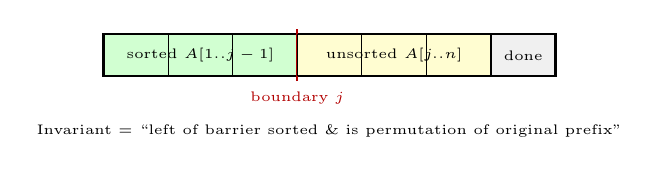
\begin{tikzpicture}[scale=0.82]
\draw[thick,fill=green!18] (0,0) rectangle (3.0,0.65);
\draw[thick,fill=yellow!18] (3.0,0) rectangle (6.0,0.65);
\draw[thick,fill=gray!12] (6.0,0) rectangle (7.0,0.65);
\draw[thick,red!70!black] (3.0,-0.08)--(3.0,0.73);
\foreach \x in {0,1,2,3,4,5,6} \draw (\x,0)--(\x,0.65);
\node[font=\tiny] at (1.5,0.32) {sorted $A[1..j-1]$};
\node[font=\tiny] at (4.5,0.32) {unsorted $A[j..n]$};
\node[font=\tiny] at (6.5,0.32) {done};
\node[font=\tiny,red!70!black] at (3.0,-0.35) {boundary $j$};
\node[font=\tiny,align=center] at (3.5,-0.85) {Invariant = ``left of barrier sorted \& is permutation of original prefix''};
\end{tikzpicture}
\end{center}
\begin{definition}[Loop invariant]
A predicate $I$ on program state is a \emph{loop invariant} for loop guard $G$ if:
\begin{enumerate}[label=(LI\arabic*)]
    \item \textbf{Initialisation:} $I$ holds before first iteration.
    \item \textbf{Maintenance:} if $I$ holds before an iteration and $G$ true, then $I$ holds after.
    \item \textbf{Termination:} $I\land\neg G$ implies desired postcondition.
\end{enumerate}
\end{definition}
Think of $I$ as the inductive hypothesis travelling around the loop---its proof \emph{is} induction on iteration count. A \emph{variant} $v$ (integer, strictly decreasing, bounded below, usually $\ge0$) guarantees termination.
\begin{example}[Insertion sort --- full correctness]
\begin{quote}\ttfamily
\textsc{InsertionSort}$(A[1\ldots n])$\\
1\ \ \textbf{for} $j\gets2$ \textbf{to} $n$ \textbf{do}\\
2\ \ \ \ \ \ $key\gets A[j]$\\
3\ \ \ \ \ \ $i\gets j-1$\\
4\ \ \ \ \ \ \textbf{while} $i>0$ \textbf{and} $A[i]>key$ \textbf{do}\\
5\ \ \ \ \ \ \ \ \ \ $A[i+1]\gets A[i]$\\
6\ \ \ \ \ \ \ \ \ \ $i\gets i-1$\\
7\ \ \ \ \ \ $A[i+1]\gets key$
\end{quote}
Spec: $A[1..n]$ is a permutation of input and non-decreasing. Outer invariant (words first): \emph{first $j-1$ slots are the original $A_0[1..j-1]$ in sorted order.} Formally $A[1..j-1]=\mathrm{sorted}(A_0[1..j-1])$. Initialisation $j=2$: $A[1..1]$ trivially sorted. Maintenance: inner loop shifts sorted block until position for $key=A_0[j]$ found, yielding sorted $A[1..j]$. Termination $j=n+1$: $A[1..n]$ sorted permutation. Inner invariant: $A[i+2..j]$ holds elements $>key$ shifted by one; $A[1..i]$ sorted. Variant $i$ decreases to $0$; outer variant $n-j$. Hence total correctness.
\end{example}
\begin{example}[Euclid terminates] Variant $v=b$: $(a,b)\mapsto(b,a\bmod b)$ with $0\le a\bmod b<b$ so $v$ strictly decreases $\ge0$. Invariant $\gcd(a,b)$ unchanged ($\gcd(a,b)=\gcd(b,a\bmod b)$) gives postcondition $a=\gcd(a_0,b_0)$. \end{example}

% ============================================================
\section{Chapter Notes}
The RAM model is due to Cook and Reckhow (1973) and Aho, Hopcroft, Ullman; our version follows CLRS Ch.~2; word-RAM is standard (Demaine). Loop invariants are Hoare logic in miniature (Hoare, 1969); full method in SC3270. For discrete math, Rosen and MH1812 notes remain references.

% ============================================================
\section{Exercises}
\label{sec:ch01-exercises}
\begin{enumerate}[label=E1.\arabic*, leftmargin=*, itemsep=0.8em]
\item \textbf{Warm-up: logic and quantifiers.} Formalise ``Every SC2001 student who passed MH1812 can follow an induction proof'' using predicates, then write its negation without $\neg$ in front of a quantifier. Why is negation \emph{not} ``No student can''?
\item \textbf{Induction --- weak vs.\ strong.} Prove $\sum_{i=1}^{n}i^2=n(n+1)(2n+1)/6$ by induction. Then prove every $n\ge12$ is $4a+5b$ ($a,b\ge0$). Which needed strong induction? (Hint: bases $12,13,14,15$.)
\item \textbf{RAM cost model.} \begin{quote}\ttfamily\textsc{SumArray}$(A[1\ldots n])$\\1\ \ $s\gets0$\\2\ \ \textbf{for} $i\gets1$ \textbf{to} $n$ \textbf{do} $s\gets s+A[i]$\\3\ \ \textbf{return} $s$\end{quote} (a) Count RAM ops/line and total time. (b) If each $A[i]$ is $b\gg\log n$ bits, how does word-RAM $w=\Theta(\log n)$ change it? (c) $O(n)$ or $O(nb/w)$?
\item \textbf{Loop invariant --- find the bug.} Invariant for \textsc{LinearSearch}: ``At start of iteration $i$, $key\notin A[1..i-1]$.'' Prove correctness if used correctly. Give a buggy variant where invariant holds but algorithm incorrect on termination; which of (LI1)--(LI3) fails?
\item \textbf{Euclid's invariant in full.} Show (a) $\gcd(a,b)=\gcd(b,a\bmod b)$ for $b>0$, (b) invariant holds/when $b=0$ postcondition, (c) $O(\log b)$ iterations via $a\bmod b<a/2$ when $b\le a$.
\end{enumerate}
% End of Chapter 1
